\section{Introduction}

\subsection{Context}

Alcohol is a legal drug in most countries worldwide, which makes it very easy to access for anyone who is over the legal age to buy it in their country.

According to organizations like the World Health Organization \cite{who}, the harmful use of alcohol is a causal factor in more than 200 disease and injury conditions and in the age group 20–39 years approximately 13.5\% of the total deaths are alcohol-attributable. Worldwide, 3 million deaths every year result from the harmful use of alcohol, a 5.3\% of all deaths \cite{whoalcohol}.

As it is shown in Figure \ref{vulnerabilities}, there are individual and societal vulnerability factors \cite{whoalcohol} that affect alcohol consumption and alcohol-related harm. In the context of the occidental world, alcohol consumption is totally accepted and most of the socialization among individuals is made by eating and drinking, being most of the beverages alcoholic ones. This could lead sometimes to a misuse and abuse of alcoholic beverages, taking bad decisions, some more naive like texting an ex-partner, some more hazardous like driving.

\begin{figure}[H]
    \centering
    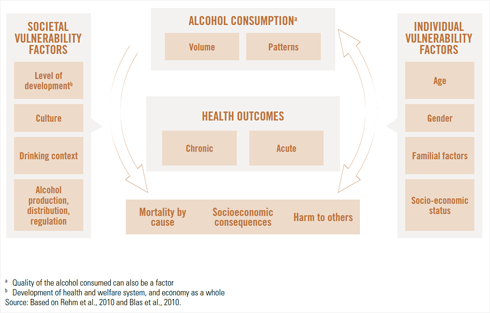
\includegraphics[width=0.9\textwidth]{./img/vulnerabilities.png}
    \caption{Vulnerabilities declared by the WHO. Reprinted from \cite{who}.}
    \label{vulnerabilities}
\end{figure}

  \subsection{Motivation}

  Nowadays, most people, at least in the developed countries, own one or more smartphones. This makes the monitoring of people easier than ever. Adding to this fact how science has advanced, it makes up one of the best possible scenarios for studying the interaction between society and alcohol intake, both amount of alcohol consumed and behavior changes.

  Having in mind what has been previously mentioned and with the exhaustive use of smartphones that is being done, the sensing of people's behaviors has been made easier, and as an example, we could use the keyboard to check whether the writing gets worse or the predictive words are used more frequently after consuming alcohol or taking a selfie to estimate the blood alcohol concentration.

  According to Medical News Today \cite{mnt} and Healthline \cite{healthline}, amoung the numerous effects on the consumer's body and behaviour, the consumption of alcohol may lead to reduced reaction and movement. This will be key aspect to be considered for the system we want to develop. As a consequence of the alcohol intoxication, an abnormal movement is shown by the eyes, known as Nystagmus.

  Nystagmus is, according to MedlinePlus \cite{Nystagmus}, 'a term to describe fast, uncontrollable movements of the eyes that may be side to side (horizontal nystagmus), up and down (vertical nystagmus) and rotary (rotary or torsional nystagmus)'. This effect is the one described in Figure \ref{nystagmuses}. Nystagmus can affect vision, balance, and coordination.

  \begin{figure}[H]
      \centering
      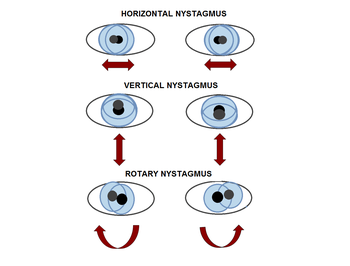
\includegraphics[width=0.45\textwidth]{./img/nystagmuses.png}
      \caption{Horizontal, vertical and rotary Nystagmus}
      \label{nystagmuses}
  \end{figure}

  \subsection{Approach and planning}


  \subsection{Objectives}
  \begin{itemize}
    \item \textbf{Main goal}: to develop a system to automatically assess a person's drunkness based on the analysis of their eye(s) movement.
    \item \textbf{Secondary goals}:
      \begin{itemize}
        \item To design a system that detects and tracks the user's eyes and analyzes them in search of horizontal nystagmus movements.
        \item To develop a system that detects and tracks the user's eyes and analyzes them in search of horizontal nystagmus movements.
        \item To evaluate and test the previously mentioned system.
      \end{itemize}
  \end{itemize}

  \subsection{Structure}

The first chapter of the project, \textit{\nameref{state}}, contains a wider perspective of the current state of tools to detect and monitorize alcohol consumption through a research about wearables, applications and scientific articles. The second chapter, \textit{\nameref{design}}, shows a more exhaustive list of the requisites of the system and the design followed: architecture, programming languages and frameworks used. The third chapter, \textit{\nameref{implementation}}, offers a detailed explanation of the development and deployment of the system. The fourth chapter, \textit{\nameref{discussion}}, analyses the system by means of System Usability Scale tests \cite{sus} and analysis of the data obtained from the use of the application. The fifth and last chapter, \textit{\nameref{conclusions}}, analyses the initial objectives of the project and whether they were achieved or not, as well as possible future work.
